% Ensemble Architecture Performance Trajectory (v1.0 → v6.0)
% Replaces: tab:performance-trajectory in appendix_m
% Shows the 13-month journey from catastrophic failure to profitability

\begin{figure}[htbp]
\centering
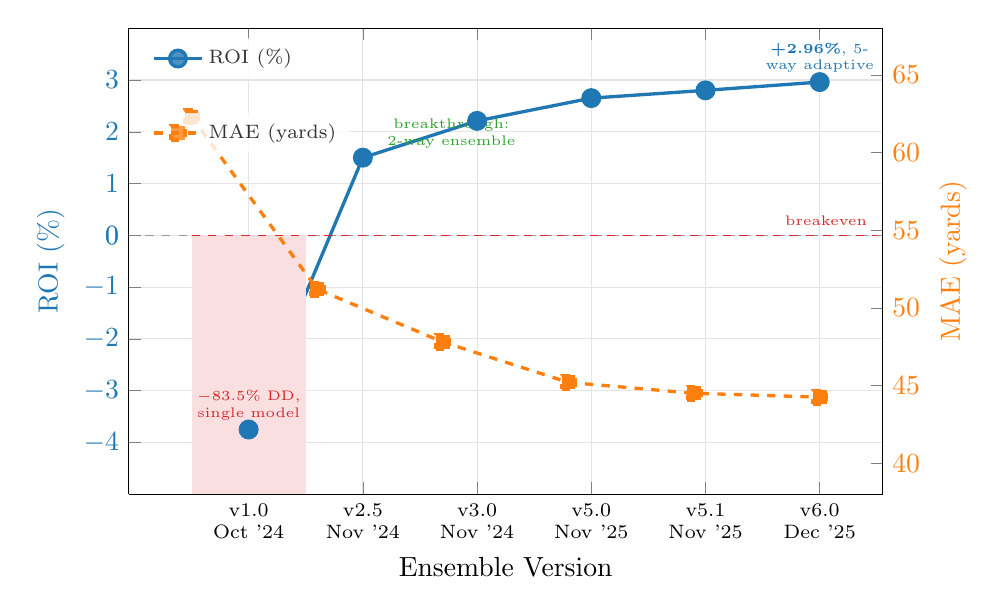
\begin{tikzpicture}
\definecolor{accent}{RGB}{31,119,180}
\definecolor{accentRed}{RGB}{214,39,40}
\definecolor{accentGreen}{RGB}{44,160,44}
\definecolor{accentOrange}{RGB}{255,127,14}

\begin{axis}[
  width=0.92\textwidth,
  height=7.5cm,
  axis y line*=left,
  xlabel={Ensemble Version},
  ylabel={ROI (\%)},
  ylabel style={color=accent},
  ymin=-5, ymax=4,
  xtick={1,2,3,4,5,6},
  xticklabels={
    {\shortstack{v1.0\\Oct '24}},
    {\shortstack{v2.5\\Nov '24}},
    {\shortstack{v3.0\\Nov '24}},
    {\shortstack{v5.0\\Nov '25}},
    {\shortstack{v5.1\\Nov '25}},
    {\shortstack{v6.0\\Dec '25}}
  },
  xticklabel style={font=\scriptsize},
  ytick={-4,-3,-2,-1,0,1,2,3},
  yticklabel style={color=accent},
  grid=major,
  grid style={gray!20},
  legend style={at={(0.02,0.98)}, anchor=north west, font=\scriptsize, draw=none, fill=white, fill opacity=0.8},
  extra y ticks={0},
  extra y tick style={grid style={black!40, dashed}},
]

% ROI line
\addplot[accent, very thick, mark=*, mark size=3pt] coordinates {
  (1, -3.75) (2, 1.50) (3, 2.21) (4, 2.65) (5, 2.80) (6, 2.96)
};
\addlegendentry{ROI (\%)}

% Shade loss region
\addplot[fill=accentRed!15, forget plot, draw=none, area legend] coordinates {
  (0.5, -5) (0.5, 0) (1.5, 0) (1.5, -5)
} -- cycle;

% Breakeven line
\draw[accentRed, dashed, thin] (axis cs:0.5,0) -- (axis cs:6.5,0);
\node[accentRed, font=\tiny, anchor=south east] at (axis cs:6.5,0) {breakeven};

% Milestone annotations
\node[font=\tiny, text=accentRed, anchor=south, align=center, text width=2cm] at (axis cs:1,-3.75)
  {$-$83.5\% DD, single model};
\node[font=\tiny, text=accentGreen, anchor=south west, align=center, text width=2cm] at (axis cs:2,1.50)
  {breakthrough: 2-way ensemble};
\node[font=\tiny, text=accent, anchor=south, text width=2cm, align=center] at (axis cs:6,2.96)
  {\textbf{+2.96\%}, 5-way adaptive};

\end{axis}

% Second y-axis: MAE
\begin{axis}[
  width=0.92\textwidth,
  height=7.5cm,
  axis y line*=right,
  axis x line=none,
  ylabel={MAE (yards)},
  ylabel style={color=accentOrange},
  ymin=38, ymax=68,
  xtick={1,2,3,4,5,6},
  xticklabels={},
  ytick={40,45,50,55,60,65},
  yticklabel style={color=accentOrange},
  legend style={at={(0.02,0.82)}, anchor=north west, font=\scriptsize, draw=none, fill=white, fill opacity=0.8},
]

% MAE line
\addplot[accentOrange, very thick, mark=square*, mark size=2.5pt, dashed] coordinates {
  (1, 62.3) (2, 51.2) (3, 47.8) (4, 45.2) (5, 44.5) (6, 44.25)
};
\addlegendentry{MAE (yards)}

\end{axis}
\end{tikzpicture}
\caption[Ensemble performance trajectory]{Ensemble architecture performance trajectory (v1.0 $\to$ v6.0). ROI transitions from catastrophic loss ($-3.75\%$) to sustained profitability ($+2.96\%$) over 13 months. MAE decreases from 62.3 to 44.25 yards ($-29\%$). The v2.5 breakthrough (first ensemble) marks the single largest improvement.}
\label{fig:ensemble-progression-chart}
\end{figure}
